\textbf{Heavy-tail} distributions, say, 
Student, Cauchy, and Laplace (double sided Exp.) distributions, 
is robust to outliers.\unsure{
Grafting of Normal main body and Cauchy tails are also used to deal with outliers like RCTD.
} 
It is common to set $\nu=4$, if greater, then Student dist. approaches to $\mathcal{N}$.

\textbf{Monte Carlo approximation}. 
Consider an arbitrary transformation $\bm{Y}=g(\bm{X})$,
it is often difficult to compute the induced distribution $f_{\bm{Y}}(\bm{y})$ analytically,
but it can be approached by drawing a large amount of samples 
from the original distribution $f_{\bm{X}}(\bm{x})$:
\begin{gather}
    f_{\hat{\bm{Y}}}(\bm{y})
    \triangleq
    \frac{1}{N}\sum_{s=1}^N\delta(\bm{y}-g(\bm{x}_s))
\end{gather}

\textbf{Simpson's paradox} says that a statistical trend or relationship 
that appears in several difficult groups of data can disappear or reverse sign 
when these groups are combined.

\textbf{Convariance} of multiple r.v.. $\bm{X}=(X_1,\cdots,X_D)$ is defined as\unsure{
Useful in Multivariate Analysis and Linear Model
} 
\begin{align}
    \bm{\Sigma}\triangleq\mathrm{Cov}\bm{X}
    =& \mathbb{E}\left[
    (\bm{X}-\mathbb{E}\bm{X})
    (\bm{X}-\mathbb{E}\bm{X})^T
    \right]\\
    =& \mathbb{E}[\bm{XX}^T]-[\mathbb{E}\bm{X}][\mathbb{E}\bm{X}]^T
\end{align}
\begin{enumerate}
    \item $\mathbb{E}[\bm{XX}^T]=\bm{\Sigma}+\bm{\mu}\bm{\mu}^T$
    \item $\mathrm{Cov}[\bm{AX}+\bm{b}]=\bm{A}\mathrm{Cov}\bm{X}\bm{A}^T$
    \item \unsure{There are some other properties of multiple r.v. waiting to be added.}
\end{enumerate}

\textbf{Multivariate Gaussian/normal} (MVN) r.v. 
$\bm{X}\sim\mathcal{N}(\bm{\mu},\bm{\Sigma})$
\begin{gather}
    f_{\bm{X}}(\bm{x})
    = \frac{1}{(2\pi)^\frac{D}{2}|\bm{\Sigma}|^\frac{1}{2}}
    \exp\left\{ 
        -\frac{1}{2}
        (\bm{x}-\bm{\mu})^T
        \bm{\Sigma}^{-1}
        (\bm{x}-\bm{\mu}) 
    \right\}
\end{gather}

\textbf{Mahalanobis distance} $\Delta$ between $\bm{x}$ and $\bm{\mu}$
under the assumption of above MVN is defined as
\begin{gather}
    \Delta^2\triangleq
    (\bm{x}-\bm{\mu})^T
    \bm{\Sigma}^{-1}
    (\bm{x}-\bm{\mu}),
\end{gather}
implying that \uline{the points with a same density have a same Mahalanobis distance 
away from the population mean point $\bm{\mu}$}, say, like contours.
It can be interpreted as Euclidean distance in a new coordinate 
from the original coordinate by the transformation of 
$\bm{\Sigma}^{-1}$,
which can be computed by eigendecomposition:
\begin{gather}
    \bm{\Sigma}
    = \sum_{d=1}^D{\lambda_d\bm{u}_d\bm{u}_d^T}
    % = \bm{U}\mathrm{diag}(\lambda_1,\cdots,\lambda_D)\bm{U}^T\\
    = \bm{U}\bm{D}\bm{U}^T\\
    \bm{\Sigma}^{-1}
    = \sum_{d=1}^D{\lambda_d^{-1}\bm{u}_d\bm{u}_d^T}
    % = \bm{U}\mathrm{diag}(\lambda_1,\cdots,\lambda_D)^{-1}\bm{U}^T
    = \bm{U}\bm{D}^{-1}\bm{U}^T
    \triangleq \bm{\Lambda}
\end{gather}
where $\bm{U}=[\bm{u}_1,\cdots,\bm{u}_D]$ is eigenvectors for rotation and 
$\bm{D}=\mathrm{diag}(\lambda_1,\cdots,\lambda_D)$ is eigenvalues for scaling.\unsure{
This procedure is similar with the standardization of univariable Gaussian.}


\textbf{Marginals and conditionals of an MVN}: \unsure{
Marginals and conditionals of a multi-variable model is important and frequently used conclusion.
}
Suppose $\bm{X}=[\bm{X}_1,\bm{X}_2]^T\sim\mathcal{N}(\bm{\mu},\bm{\Sigma})$, where
\begin{gather}
    \bm{\mu}=\left[\begin{array}{c}
        \bm{\mu}_1 \\
        \bm{\mu}_2
    \end{array}\right],~
    \bm{\Sigma}=\left[\begin{array}{cc}
        \bm{\Sigma}_{11} & \bm{\Sigma}_{12} \\
        \bm{\Sigma}_{21} & \bm{\Sigma}_{22}
    \end{array}\right],~\text{and}~
    \bm{\Lambda}
    =\bm{\Sigma}^{-1}=\left[\begin{array}{cc}
        \bm{\Lambda}_{11} & \bm{\Lambda}_{12} \\
        \bm{\Lambda}_{21} & \bm{\Lambda}_{22}
    \end{array}\right]
\end{gather}
is the \textbf{precision matrix}.
$\Rightarrow$
\begin{align}
    \bm{X}_1
    \sim& \mathcal{N}(\bm{\mu}_1,\bm{\Sigma}_{11}),\\
    \bm{X}_1|\bm{X}_2
    \sim& \mathcal{N}
    (\bm{\mu}_{1|2},\bm{\Sigma}_{1|2})
\end{align}
where 
\begin{align}
    \bm{\mu}_{1|2}
    =& \bm{\Sigma}_{1|2}
    [\bm{\Lambda}_{11}\bm{\mu}_1
    -\bm{\Lambda}_{12}(\bm{X}_2-\bm{\mu}_2)],\\
    \bm{\Sigma}_{1|2}
    =& \bm{\Sigma}_{11}
    -\bm{\Sigma}_{12}\bm{\Sigma}_{22}^{-1}\bm{\Sigma}_{21}
    =\bm{\Lambda}_{11}^{-1}.
\end{align}

% \begin{example}
%     $~$\\
%     $\bm{\Sigma}=\left[\begin{array}{cc}
%         \sigma_1^2 & \rho\sigma_1\sigma_2 \\
%         \rho\sigma_1\sigma_2 & \sigma_2^2
%     \end{array}\right]$, and compute the marginal and conditional distribution.
% \end{example}

\begin{example}
    \textbf{Missing value imputation}\\
    infer the missing entries 
    by exploiting the correlation (in $\bm{\Sigma}$) amongst the dimensions,
    say, computing 
    $p(\bm{x}_{n,\bm{h}}|\bm{x}_{n,\bm{v}},\bm{\theta})$
    and obtain the posterior mean (optimally guessed values) and variance (confidence measure).
\end{example}


\textbf{Linear Gaussian system}.
Let $\bm{Z}\in\mathbb{R}^L$ be an unknown vector of values, 
and $\bm{Y}\in\mathbb{R}^D$ be some \textbf{noisy measurement} of $\bm{Z}$:
\begin{align}
    \bm{Z}
    \sim& \mathcal{N}(\bm{\mu}_z,\bm{\Sigma}_z)\\
    \bm{Y}|\bm{Z}=\bm{z}
    \sim& \mathcal{N}(\bm{Wz}+\bm{b},\bm{\Sigma}_y)
\end{align}
The joint distribution of $[\bm{Z},\bm{Y}]$ follows is Gaussain 
$\mathcal{N}(\bm{\mu},\bm{\Sigma})$, where\unsure{
The unconditional variance of $\bm{Y}$ includes its conditional variance, $\bm{\Sigma}_y$,
and the squared weight-scaled variance of $\bm{Z}$, $\bm{W\Sigma}_z\bm{W}^T$.
}
\begin{gather}
    \bm{\mu}
    = \left[\begin{array}{c}
        \bm{\mu}_z \\
        \bm{W\mu}_z+\bm{b} 
    \end{array}\right],~
    \bm{\Sigma}
    = \left[\begin{array}{cc}
        \bm{\Sigma}_z & \bm{\Sigma}_z\bm{W}^T \\
        \bm{W\Sigma}_z & \bm{\Sigma}_y+\bm{W\Sigma}_z\bm{W}^T
    \end{array}\right]
\end{gather}

\begin{example}
    \textbf{relationship from observations to latent factors}\\
    Infer the \uline{relationship from observations to latent factors}: $\bm{Y}\to\bm{Z}$ by Bayes rule:
    \begin{align}
        \bm{Y}
        \sim& \mathcal{N}(\bm{W\mu}_z+\bm{b},\bm{\Sigma}_y+\bm{W\Sigma}_z\bm{W}^T)\\
        \bm{Z}|\bm{Y}=\bm{y}
        \sim& \mathcal{N}(\bm{\mu}_{z|y},\bm{\Sigma}_{z|y}),
    \end{align}
    where
    \begin{align}
        \bm{\mu}_{z|y}
        =& \bm{\Sigma}_{z|y}\left[
            \bm{W}^T\bm{\Sigma}_y^{-1}(\bm{y}-\bm{b})+\bm{\Sigma}_z^{-1}\bm{\mu}_z
        \right]~\text{and}~\\
        \bm{\Sigma}_{z|y}^{-1}
        =& \bm{\Sigma}_z^{-1}+\bm{W}^T\bm{\Sigma}_y^{-1}\bm{W}
    \end{align}
\end{example}

\begin{example}
    \textbf{shrinkage} and \textbf{Singal-to-noise ratio}\\
    Suppose $Y_i=Z+\varepsilon$ is the observed signal with 
    $\varepsilon\sim\mathcal{N}(0,\Sigma_y)$ and
    $Y_i|Z=z\sim\mathcal{N}(z,\Sigma_y)$,
    and $z\sim\mathcal{N}(\mu_0,\Sigma_0)$ is the true signal, 
    then $Z|\bm{y}\sim\mathcal{N}(\mu_N,\Sigma_N)$, where
    \begin{align}
        \Sigma_N
        =& \left(\Sigma_0^{-1}+N\Sigma_N^{-1}\right)^{-1}\\
        \mu_N
        % =& \frac{\Sigma_y/N}{\Sigma_0+\Sigma_y/N}\mu_0+\frac{\Sigma_0}{\Sigma_0+\Sigma_y/N}\Bar{y}_N\\
        % =& \mu_0 + ({\Bar{y}_N-\mu_0})\frac{\Sigma_0}{\Sigma_y/N+\Sigma_0}\\
        =& \Bar{y}_N - (\Bar{y}_N-\mu_0)\frac{\Sigma_y/N}{\Sigma_y/N+\Sigma_0} \label{eq:shrinkage}
    \end{align}
    The data is adjusted towards the prior mean with the increasing of noise deviation, called \textbf{shrinkage}, by Equation (\ref{eq:shrinkage}).
    And the amount of shrinkage is defined as \textbf{signal-to-noise ratio}, 
    \begin{gather}
        \text{SNR}\triangleq\frac{\mathbb{E}Z^2}{\mathbb{E}\varepsilon^2}=\frac{\Sigma_0+\mu_0^2}{\Sigma_y}
    \end{gather}
    By increasing the number of observations, 
    the SNR can be amplified through reducing the variance of noise $\varepsilon$, 
    and this conclusion can be extend to multi-variable case.
\end{example}
% \unsure{
%     recall the convex combination of the prior and the data
%     }
\begin{example}
    \textbf{Senser fusion}\\
    There are $M$ sensors (measurement devices) and $N_m$ observations for each devices, 
    the the signals $Y_{1,m},\cdots,Y_{n,m},\cdots,Y_{N_m,m}|\bm{Z}=\bm{z}\overset{iid}{\sim}\mathcal{N}(\bm{z},\Sigma_m)$. Sensor fusion is to combine the evidence together, to compute $p(\bm{z}|\bm{y})$.
\end{example}

\begin{question}
    Why is exponential family so important?
\end{question}

\textbf{Maximum entropy derivation of the exponential family}:
Recall \textbf{KL divergence} of two distributions, $p$ and $q$, not symmetric
\begin{gather}
    \infdiv{p}{q}
    \triangleq\left\{
    \begin{array}{ll}
        \int_\mathcal{X}{p(x)\log\frac{q(x)}{p(x)}}dx & X~\text{continuous} \\
        \sum_x{p(x)\log\frac{p(x)}{q(x)}} & X~\text{discrete}
    \end{array}\right.
\end{gather}
To find a distribution $p$ that minimizes the $\infdiv{p}{q}$ with a given priori $q$
with moments constraints of observed data
\begin{gather}
    p^*=\argmin_p\infdiv{p}{q}\\
    \mathrm{s.t.}~\sum_x{p(x)}=1
    ~\text{and}~
    \sum_x{p(x)f_k(x)}=F_k,~k=1,\cdots,K
\end{gather}
The Lagrangian is given by
{\small\begin{gather}
    J(p,\bm{\lambda})
    =- \sum_x{p(x)\log\frac{p(x)}{q(x)}}
    + \lambda_0\left[1-\sum_x{p(x)}\right]
    + \sum_k{\lambda_k\left[ F_k-\sum_x{p(x)f_k(x)} \right]}\\
\Rightarrow
    p^*(x)=\frac{1}{Z}q(x)\exp\left\{-\sum_k{\lambda_kf_k(x)}\right\}
\end{gather}}
which is exactly the form of exponential family and where $Z$ is the normalization term.
e.g. if $f_1(x)=x$ and $f_2(x)=x^2$, then the best distribution with minimum KL divergence 
(or maximum entropy) and matching the observed first and second moments is Gaussian distribution.

\textbf{Gaussain mixture model} (GMM) or \textbf{mixture of Gaussian} (MoG): 
the probability of each data point $\bm{y}_n$\unsure{
Are the proportion $\pi_k$'s different for each data points?
What is the relationship between $r_{nk}$ and $\pi_k$ in Equation (\ref{eq:mogpir})?
} is determined 
by certain weights of multiple distinct Gaussian models,
often used for clustering, e.g. K-means with $\bm{\Sigma}_k=\bm{I}$, $k=1,\cdots,K$.
\begin{gather}
    p(\bm{y}|\bm{\theta})=\sum_{k=1}^K{\pi_k\mathcal{N}(\bm{\mu}_k,\bm{\Sigma}_k)}
\end{gather}
\begin{align}
    \hat{\bm{\theta}}
    =& \argmax_{\bm{\theta}}\log{p(\bm{y}_1,\cdots,\bm{y}_N|\bm{\theta})}~\text{(by MLE)}\\
    \hat{\pi}_{nk}
    \overset{?}{=}& r_{nk}\triangleq p(z_n=k|\bm{y}_n,\hat{\bm{\theta}}) \label{eq:mogpir}\\
    =& \frac{p(z_n=k|\hat{\bm{\theta}})p(\bm{y}_n|z_n=k,\hat{\bm{\theta})z}}
    {\sum_{k'=1}^K{p(z_n=k'|\hat{\bm{\theta}})p(\bm{y}_n|z_n=k',\hat{\bm{\theta})}}}~\text{(by Bayes)}
\end{align}
\unsure{
The optimization process of EM or SGD will be discussed in \citep{pml1Book}, Chapter 8.
}

\textbf{Bernoulli mixture model} (BMM) or \textbf{mixture of Bernoullis} (MoB):
similar with MoG:
\begin{gather}
    p(\bm{y}|\bm{\theta})=\sum_{k=1}^K{\pi_k\underbrace{\prod_{d=1}^D\mathrm{Ber}(y_d|\mu_{dk})}_{\text{proba. of r. vec.}}}
\end{gather}

\textbf{Ordered Markov property} in a \textbf{Bayesian network} is that 
each node $Y_i$ is conditionally independent of all its predecessors ($\bm{Y}_{\text{pre}(i)}$) given its parents ($\bm{Y}_{\text{par}(i)}$):
\begin{gather}
    Y_i\perp\bm{Y}_{\text{pre}(i)\setminus\text{par}(i)}|\bm{Y}_{\text{par}(i)}\\
    p(\bm{Y}_{1:N_G})=\prod_{i=1}^{N_G}p\left(Y_i|\bm{Y}_{\text{par}(i)}\right)
\end{gather}
where $p\left(Y_i|\bm{Y}_{\text{par}(i)}\right)$ is called \textbf{conditional probability distribution} (CPD), 
which can be written as the conditional probability table (CPT) 
when the status of each node is (discrete) categorical distribution.
In Markov chain model, 
$p(y_t|y_{t-1})$ is called \textbf{transition function/kernel} (or \textbf{state transition matrix} in the case of discrete status) and is \textbf{stationary/time-invariant} under the assumption that $p(y_t|y_{t-1})$ is the same for all time steps.

\begin{figure}[hptb]
    \centering
    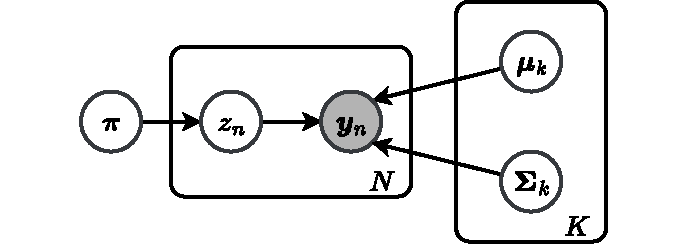
\includegraphics[width=0.5\textwidth]{figs/mixgaussian.pdf}
    \caption{A Gaussian mixture model represented as a graphical model}
    \label{fig:maxgaussian}
\end{figure}

\begin{example}
    \textbf{GMM represented as a graphical model}\\
    Viewing all variables, including model's parameters and obverations, 
    follow a generative story like Figure (\ref{fig:maxgaussian})
    {\small\begin{gather}
        p(\bm{y}_{1:N},\bm{z}_{1:N},\bm{\theta})
        = p(\bm{\pi})
        \left[ \prod_{k=1}^K p(\bm{\mu}_k)p(\bm{\Sigma}_k) \right]
        \left[ \prod_{n=1}^N p(z_n|\bm{\pi})p(\bm{y}_n|z_n,\bm{\mu}_{1:K},\bm{\Sigma}_{1:K}) \right]
    \end{gather}}
    where latent variable $z_n\sim\text{Cat}(\bm{\pi})$ and model's parameters
    $\bm{\theta}=(\bm{\pi},\bm{\mu}_{1:K},\bm{\Sigma}_{1:K})$ are all unknown.
\end{example}


\subsection{Statistics}

\begin{question}
    Why can MLE be used so uniformly?
\end{question}

\textbf{Maximum likelihood estimation} (MLE) and \textbf{maximum a posterior estimation} (MAP):
$\hat{\bm{\theta}}_{MLE}$ -- the parameters' estimation that assign the highest probability to the observations;
$\hat{\bm{\theta}_{MAP}}$ -- the parameters' estimation maximizing the posterior probability under some priori $\pi(\bm{\theta})$. 
If \uline{the priori is a uniform distribution}, 
then $\hat{\bm{\theta}}_{MLE}=\hat{\bm{\theta}}_{MAP}$.\unsure{
Reason 1
}
\begin{gather}
    \hat{\bm{\theta}}_{MLE}
    \triangleq \argmax_{\bm{\theta}}p(\mathcal{D}|\bm{\theta})\\
    \hat{\bm{\theta}}_{MAP}
    \triangleq \argmax_{\bm{\theta}}p(\bm{\theta}|\mathcal{D})
    = \argmax_{\bm{\theta}}p(\mathcal{D}|\bm{\theta})\pi(\bm{\theta})
\end{gather}
\textbf{Kullback Leibler divergence} (KL divergence): 
A standard way to measure the dissimilarity between probability distribution $p$ and $q$.
\begin{align}
    \infdiv{p}{q}
    =& \sum_{\bm{y}}{p(\bm{y})\log\frac{p(\bm{y})}{q(\bm{y})}}\\
    =& \underbrace{\sum_{\bm{y}}{p(\bm{y})\log p(\bm{y})}}_{-\mathbb{H}(p)\text{:entropy}}
    - \underbrace{\sum_{\bm{y}}{p(\bm{y})\log q(\bm{y})}}_{-\mathbb{H}_{\text{CE}}(p,q)\text{:cross-entropy}}
\end{align}
If \uline{$q(\bm{y})=p(\bm{y}|\bm{\theta})$ and $p(\bm{y})=p_\mathcal{D}(\bm{y})$}, 
then $\infdiv{p}{q}=\text{const}+\mathrm{NNL}(\bm{\theta})$.\unsure{Reason 2}
which shows the relationship between MLE and KL divergence.
And above all justify usage of MLE from the perspectives of Bayesain and empirical distribution.

\begin{example}
    \textbf{MLE for linear regression} aka\\
    \textbf{ordinary least squares} or OLS estimate
    \begin{align}
        p(y|\bm{x};\bm{\theta})
        =& \mathcal{N}(\bm{w}^T\bm{x},\sigma^2)\\
        \hat{\bm{w}}_{OLS}\equiv\hat{\bm{w}}_{MLE}
        \triangleq& \argmin_{\bm{w}}\text{NLL or RSS or MSE or RMSE}\\
        =& (\bm{X}^T\bm{X})^{-1}\bm{X}^T\bm{y}
    \end{align}
\end{example}

\textbf{Empirical risk minimization} (ERM) 
\begin{gather}
    \mathcal{L}(\bm{\theta})=\frac{1}{N}\sum_{n=1}^N\ell(\bm{y}_n,\bm{\theta};\bm{x}_n)
\end{gather}
where $\ell(\cdot)$ is any loss function that measures the mismatchness with expected outcomes, 
(if $\ell(\bm{y}_n,\bm{\theta};\bm{x}_n)=-\log{p(\bm{y}_n|\bm{\theta},\bm{x}_n)}$,
then $\mathcal{L}(\bm{\theta})=\text{NLL}(\bm{\theta})$ and ERM is MLE).\unsure{Reason 3}
% \textbf{Surrogate loss function}: 
% The surrogate is usually chosen to be a maximally tight
% convex upper bound, which is then easy to minimize, e.g. 

% \begin{enumerate}[(i)]
%     \item 0-1 loss: 
%     $\ell_{01}(\bm{y}_n,\bm{\theta};\bm{x}_n)=\mathbb{I}(\bm{y}_n\neq f(\bm{x}_n;\bm{\theta})$
%     \item :
    
% \end{enumerate}

\begin{figure}[hptb]
    \centering
    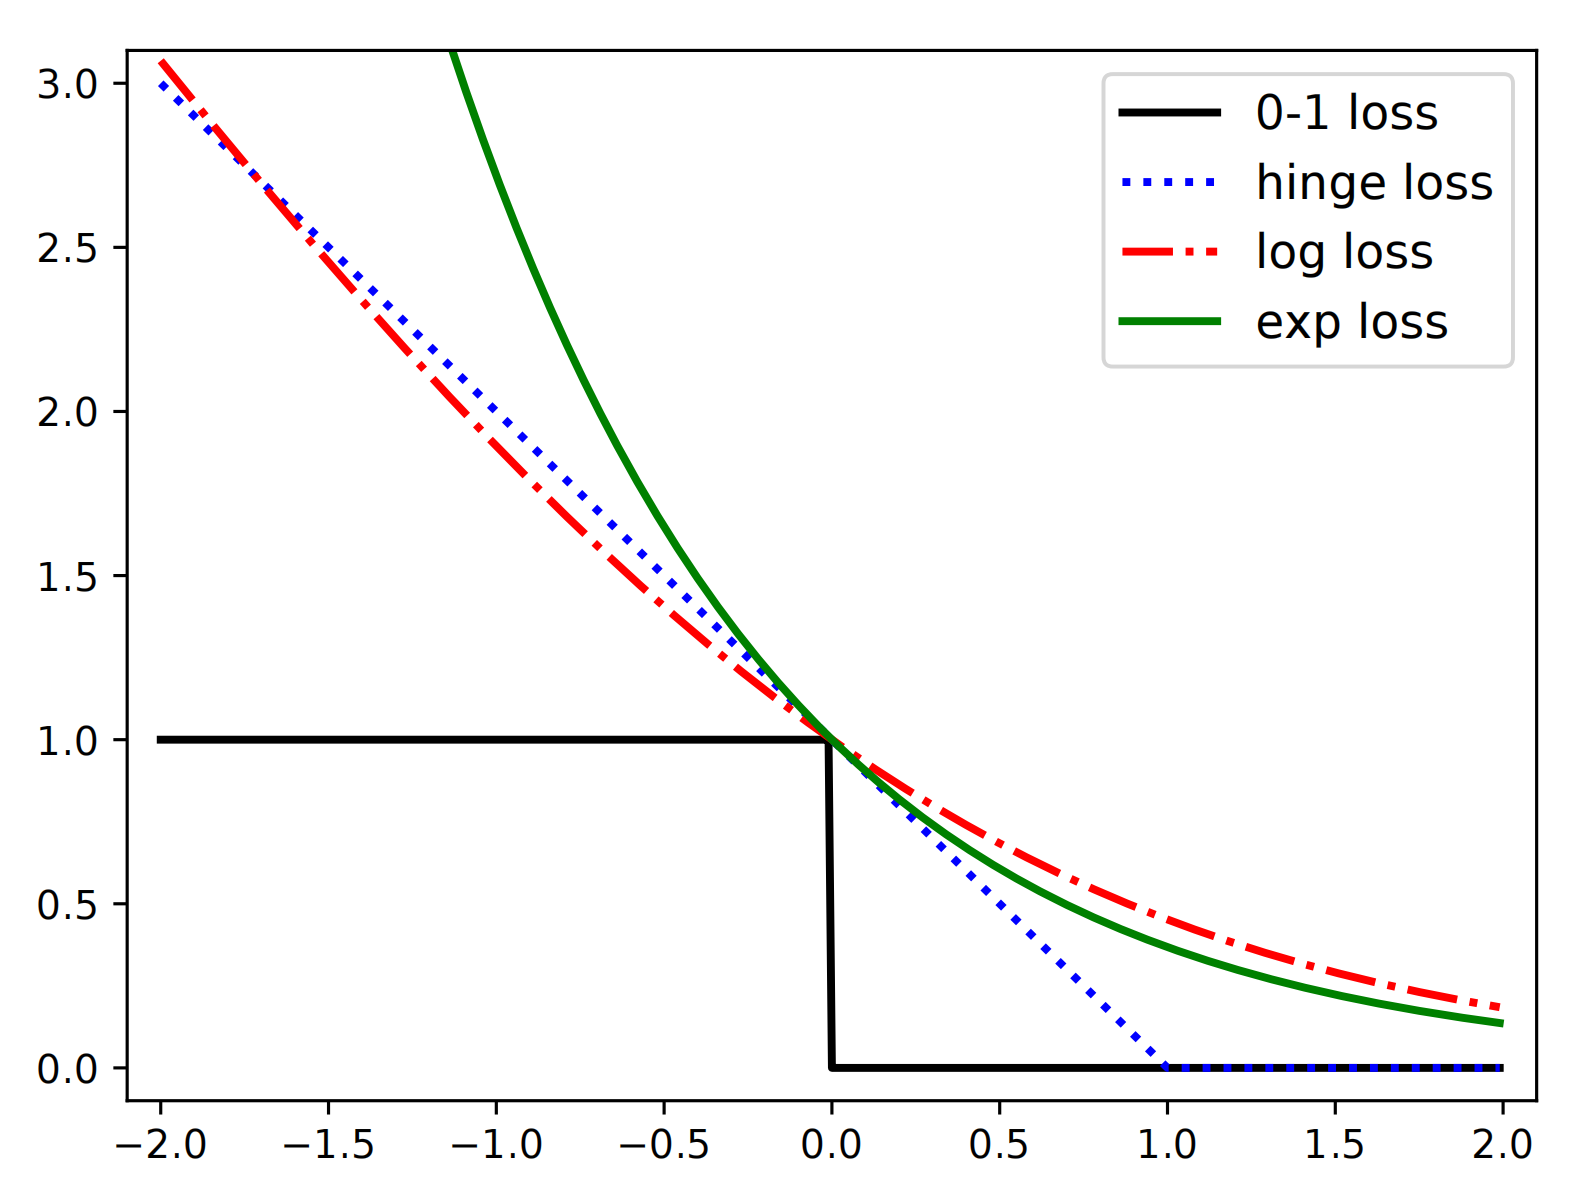
\includegraphics[width=0.5\textwidth]{figs/lossfunc.png}
    \caption{Loss functions for \uline{binary classifiers}}
    {\footnotesize Horizontal axis: $z=yf(\bm{x};\bm{\theta})$. \\
    0-1 loss: $\mathbb{I}(z<0)$;
    Hinge loss: $\max\{0,1-z\}$;
    Log-loss: $\log_2{(1+e^{-z})}$;
    Exp-loss: $e^{-z}$.}
    \label{fig:lossfunc}
\end{figure}

\textbf{Estimation method of moments} (MOM): 
equate the \uline{theoretical moments (functions of parameters)},
to the \uline{empirical moments},
where we need the same number of simultaneous equations for solving $K$ unknown parameters,
to avoid difficult computation in MLE 
but with less efficiency of data usage, so can be used to initialize iterative algorithms for MLE.

\textbf{Online (recursive) estimation} with recursive update $f$:
\begin{gather}
    \hat{\bm{\theta}}_t=f(\hat{\bm{\theta}}_{t-1},\bm{y}_t)
\end{gather}

\begin{example}
    \textbf{Exponentially-weighted moving average} (EWMA)
    \begin{align}
        \hat{\bm{\mu}}_t
        =& \beta\hat{\bm{\mu}}_{t-1}+(1-\beta)\hat{\bm{y}}_t\\
        =& \beta^t\bm{y}_0 + (1-\beta)\beta^{t-1}\bm{y}_1 + \cdots + (1-\beta)\beta\bm{y}_{t-1} + (1-\beta)\bm{y}_t
    \end{align}
    where a smaller $\beta$ forgets the past data more quickly and 
    adapts to the more recent data more rapidly.
\end{example}

\textbf{Regularization} term $C(\bm{\theta})$ in the loss function is 
a given measure for the parameters' complexity to avoid overfitting:
\begin{gather}
    \mathcal{L}(\bm{\theta};\lambda)
    = \frac{1}{N}\sum_{n=1}^N\ell(\bm{y}_n,\bm{\theta};\bm{x}_n)
    + \lambda C(\bm{\theta})
\end{gather}
where $C(\bm{\theta})$ can be some $-\log{\pi(\bm{\theta})}$,
then objective become a MAP estimation for a given priori $\pi(\bm{\theta})$ for $\lambda=1$.
e.g. add-one smoothing (or \textbf{Laplace's rule of succession}) in Bernoulli distribution with $\pi\sim\text{Beta}(2,2)$ and shrinkage estimation for $\Sigma$ in multivariate Gaussian with $\pi\sim$ inverse Wishart. 

\textbf{Bayes model averaging} (BMA): make predictions under the posterior distribution of parameters, which weighted the predictions for all possible parameters (models)
\begin{gather}
    \pi(\bm{\theta}|\mathcal{D})
    = \frac{\pi(\bm{\theta})p(\mathcal{D}|\bm{\theta})}{p(\mathcal{D})}\\
    p(\bm{y}|\bm{x},\mathcal{D})
    = \int{p(\bm{y}|\bm{x};\bm{\theta})\pi(\bm{\theta}|\mathcal{D})}d\bm{\theta}
\end{gather}
where $\bm{x}$ is new observations, $\mathcal{D}$ is training data, and 
$p(\bm{y}|\bm{x},\mathcal{D})$ is the final averaging model.


\textbf{Mixtures of priors} by introducing a latent indicator variable $h$
\begin{gather}
    \pi(\bm{\theta})=\sum_k p(h=k)\pi(\bm{\theta}|h=k)
\end{gather}
$\Rightarrow$
\begin{align}
    \pi(\bm{\theta}|\mathcal{D})
    =& \sum_k{p(h=k|\mathcal{D})p(\bm{\theta}|\mathcal{D},h=k)}\\
    p(h=k|\mathcal{D})
    =& \frac{p(h=k)p(\mathcal{D}|h=k)}{\sum_{k'}{p(h=k')p(\mathcal{D}|h=k')}}
\end{align}
\unsure{
The detailed discussion on 
prior, posterior, predictive, and marginal likelihood of
(1) Beta-Binomial, (2)\textbf{Dirichlet-Multinomial}, and (3) Gaussian-Gaussian
are skipped.
}

\textbf{Other priors} besides conjugate priors
\begin{enumerate}[(1)]\label{kspt:noninfo}
    \item \textbf{noninformative prior} or preferred \textbf{minimally informative prior}: 
    let the data speak for itself, 
    e.g. \textbf{flat prior} $\pi\propto 1$ in Gaussian;
    \item \textbf{hierarchical prior}: the hyperparameters in prior also follow some prior --
    $\bm{\phi}\to\bm{\theta}\to\mathcal{D}$;
    \item \textbf{empirical prior}: the prior's hyperparameters $\bm{\phi}$ directly estimated from data $\mathcal{D}$ as shown below
    \begin{gather}
        \hat{\bm{\phi}}(\mathcal{D})
        = \argmax_{\bm{\phi}}p(\mathcal{D}|\bm{\phi})
        = \argmax_{\bm{\phi}}\int{p(\mathcal{D}|\bm{\theta})p(\bm{\theta}|\bm{\phi})}d\bm{\theta}
    \end{gather}
    which is called \textbf{Empirical Bayes} (EB).
\end{enumerate}

Available inference methods:
\begin{itemize}
    \item MLE:
    \begin{gather}
        \hat{\bm{\theta}}
    =\argmax_{\bm{\theta}}
    p(\mathcal{D}|\bm{\theta})
    \end{gather}
    \item MAP: 
    \begin{gather}
        \hat{\bm{\theta}}
    =\argmax_{\bm{\theta}}
    p(\mathcal{D}|\bm{\theta})p(\bm{\theta}|\bm{\phi})
    \end{gather}
    \item MLE-II (EB):
    \begin{gather}
        \hat{\bm{\phi}}
    =\argmax_{\bm{\phi}}
    \int{p(\mathcal{D}|\bm{\theta})p(\bm{\theta}|\bm{\phi})}d\bm{\theta}
    \end{gather}
    \item MAP-II:
    \begin{gather}
        \hat{\bm{\phi}}
    =\argmax_{\bm{\phi}}
    \int{p(\mathcal{D}|\bm{\theta})p(\bm{\theta}|\bm{\phi})p(\bm{\phi})}d\bm{\theta}
    \end{gather}
    \item Full Bayes:
    \begin{gather}
        p(\bm{\theta},\bm{\phi}|\mathcal{D})
    \propto p(\mathcal{D}|\bm{\theta})p(\bm{\theta}|\bm{\phi})p(\bm{\phi})
    \end{gather}
\end{itemize}

\textbf{Computational issues} in Bayesian ML: 
It is usually \uline{intractable to compute $p(\bm{\theta}|\mathcal{D})$}
given $p(\mathcal{D}|\bm{\theta})$ and $p(\bm{\theta})$.
Therefore, methods of \textbf{approximate posterior inference} are necessary.
\begin{itemize}
    \item \textbf{Grid approximation}:  
    brute-force enumerate finite set in partition the space of possible values $\bm{\theta}$.
    \begin{gather}
        p(\bm{\theta}=\bm{\theta}_k|\mathcal{D})
        \approx \frac{p(\mathcal{D}|\bm{\theta}_k)}{\sum_{k'=1}^K{p(\mathcal{D},\bm{\theta}_{k'})}}
    \end{gather}
    \item \textbf{Quadratic (Laplace) approximation}: 
    approximate the posterior by a multivariable Gaussian.
    $\mathcal{E}(\bm{\theta})=-\log{p(\bm{\theta},\mathcal{D})}$ is an \textbf{energy function}, 
    $\hat{\bm{\theta}}$ is the mode ($\Rightarrow\nabla{\mathcal{E}(\bm{\theta})}|_{\bm{\theta}=\hat{\bm{\theta}}}=\bm{0}$), 
    at which $\mathbf{H}$ is Hessian of $\mathcal{E}$.
    \begin{gather}
        p(\bm{\theta}|\mathcal{D})
        \approx \mathcal{N}(\hat{\bm{\theta}},\mathbf{H}^{-1})
    \end{gather}
    \item \textbf{Variational approximation}: 
    find a $q$ minimizing \uline{some discrepancy $D$}, say KL divergence, with target posterior
    in tractable family of distribution $\mathcal{Q}$,
    \begin{gather}
        p(\bm{\theta}|\mathcal{D})
        \approx q^*=\argmin_{q\in\mathcal{Q}} \infdiv{q}{p}
    \end{gather}
    \item \textbf{Monte Carlo approximation}: 
    build an empirical distribution of $\bm{\theta}$ by
    \uline{efficiently create a postrior sample of parameters} $\{\Tilde{\bm{\theta}}_s\}_{s=1}^S\sim p(\bm{\theta}|\mathcal{D})$, 
    without having to evaluate the normalization constant $p(\mathcal{D})$, then
    \begin{gather}
        p(\bm{\theta}|\mathcal{D})
        \approx\frac{1}{S}\sum_{s=1}^S\delta(\bm{\theta}-\Tilde{\bm{\theta}}_s)
    \end{gather}
\end{itemize}

\textbf{Uncertainty represented by \textit{frequentist}}:
$\hat{\bm{\theta}}=\pi(\mathcal{D})$ the estimator's distribution,
\textbf{sampling distribution},
depends on the random data and it is also a r.v..\unsure{
This idea is the same with what we have learnt in STAT5010 for all estimator, 
function of observations, of some transformation of true parameter $g(\bm{\theta})$.
}
However, in the view of frequentist, 
there exists a true single value $\bm{\theta}^*$ that generates the data $\mathcal{D}\sim p(\bm{x}|\bm{\theta}^*)$.
We can find the distribution of $\hat{\bm{\theta}}$, 
$p(\pi(\mathcal{D})=\bm{\theta}|\mathcal{D}\sim\bm{\theta}^*)$ analytically if it is tractable.
If the transformation is intractable, computational issues occur, like in Bayes ML above, and 
then approximation methods are also needed.
\begin{itemize}
    \item \textbf{Gaussian approximation}: \unsure{
    Gaussian approximation is applied in C-SIDE to model the uncertainty of $\hat{\bm{\beta}}$ for testing $H_0:\bm{\beta}^*=0$}
    by the asymptotic normality of CLT (Theorem \ref{thm:asymnorm}), the distribution of MLE converges to Gaussain
    \begin{gather}
        p(\pi(\mathcal{D})=\bm{\theta}|\mathcal{D}\sim\bm{\theta}^*)
        \to
        \mathcal{N}(\bm{\theta}^*,1/N\mathbf{I}(\bm{\theta}^*))
    \end{gather}
    \item \textbf{(Non-parametric) bootstrap approximation}: a kind of MC technique,
    the distribution of $\hat{\bm{\theta}}$ is approximated 
    by the \uline{empirical distribution from observed data}:
    \begin{gather}
        p(\pi(\mathcal{D})=\bm{\theta}|\mathcal{D}\sim\bm{\theta}^*)
        \approx \frac{1}{S}\sum_{s=1}^S\delta(\bm{\theta}-\pi(\Tilde{\mathcal{D}}_s))
    \end{gather}
    The key of bootstrap is to sample $S$ new datasets $\{\Tilde{\mathcal{D}}_s\}$ with the same size with and from the original dataset,
    $\Tilde{\mathcal{D}}$, with replacement.
    $N:=|\Tilde{\mathcal{D}}|=|\Tilde{\mathcal{D}}_s|$,
    the probability an item is picked at least once is 
    $1-\left(1-\frac{1}{N}\right)^N\to1-e^{-1}$.\unsure{
    Relationship sampling distribution and posterior distribution:
    recall the minimally informative prior in $\S$ \ref{kspt:noninfo}. 
    Sampling distribution only relies on the data.
    }
\end{itemize}


\begin{theorem}\label{thm:asymnorm}
    \textbf{Asymptotic normality}\footnote{
    \citep{pml1Book} Thm 4.7.1
    }\\
    If the parameters are identifiable, then
    \begin{gather}
        p(\pi(\mathcal{D})=\bm{\theta}|\mathcal{D}\sim\bm{\theta}^*)
        \to
        \mathcal{N}(\bm{\theta}^*,1/N\mathbf{I}(\bm{\theta}^*))
    \end{gather}
    where $\mathbf{I}(\bm{\theta}^*)$ is the \textbf{Fisher information matrix} defined as
    \begin{gather}
        \mathbf{I}(\bm{\theta})
        \triangleq\mathbb{E}_{\bm{X}|\bm{\theta}}\left[ 
            (\nabla_{\bm{\theta}}\log{p(\bm{X}|\bm{\theta})})
            (\nabla_{\bm{\theta}}\log{p(\bm{X}|\bm{\theta})})^T
        \right]
    \end{gather}
\end{theorem}

\begin{theorem}
    \textbf{Log-likelihood with twice differentiability}\footnote{
    \citep{pml1Book} Thm 4.7.2
    }\\
    If $\log p(\bm{X}|\bm{\theta})$ is twice differentiable, and under certain regularity conditions,
    \begin{gather}
        \mathbf{I}(\bm{\theta})
        =-\mathbb{E}_{\bm{X}|\bm{\theta}}\left[ 
            (\nabla_{\bm{\theta}}^2\log{p(\bm{X}|\bm{\theta})})
        \right]
    \end{gather}
    which is \uline{Hessian of NLL}.
    \uline{A log-likelihood function with high curvature (large Hessian) will result in
    a low variance estimate, since the parameters are ``well determined'' by the data,
    and hence robust to repeated sampling.}
\end{theorem}\unsure{
Good intuitive understanding. This theorem is also introduced in STAT5010.
}



\textbf{Difference between \uline{credible interval} and \uline{confidence interval}}:
Credible interval: $\mathcal{D}$ fixed (since observed), $\theta$ random;
confidence interval: $\mathcal{D}$ random, $\theta^*$ fixed.
Confidence interval $I(\Tilde{\mathcal{D}})$ such that $P(\theta^*\in I(\Tilde{\mathcal{D}})|\Tilde{\mathcal{D}}\sim\theta^*)=0.95$ \textbf{\textit{does not}} mean that
the true parameter $\theta^*$ is 95\% likely to live inside $I(\Tilde{\mathcal{D}})$, 
which, however, is exactly the quantity given by credible interval {\color{red}$P(\theta\in I|\mathcal{D})$}.
Confidence interval will cover the true parameter $100(1-\alpha)\%$ of the time.\unsure{
very confusing concept that I still do not understand...
}

% \begin{example}
%     \mathcal{D}=(y_1,y_2) from 
%     \begin{gather}
%         p(y|\theta)=\begin{array}{ll}
%             0.5 & \text{if}~y=\theta \\
%             0.5 & \text{if}~y=\theta+1 \\
%             0 & \text{otherwise}
%         \end{array}
%     \end{gather}
%     If $\theta=39$ and we will obtain the each of data, 
%     $\{(39,39),(39,40),(40,39),(40,40)\}$, 
%     with proba. 0.25
    
% \end{example}

% \textbf{Bias-variance trade-off}


% \textbf{Confidence interval}: uncertainty of a parameter estimate.
% It is worth noting that $p(\pi(\mathcal{D})=\bm{\theta}|\mathcal{D}\sim\bm{\theta}^*)$ 
% is not distribution of true $\bm{\theta}^*$ (with not uncertainty)
% but a guess (r.v.) from data with certain change covering the unknown true $\bm{\theta}^*$.
% \textbf{$100(1-\alpha)\%$ confidence interval} is \uline{any} interval\unsure{
% recall credable region
% }

